\documentclass{article}
\usepackage[utf8]{inputenc}
\usepackage{hyperref}
\usepackage[T1]{fontenc}
\usepackage{lmodern}
\usepackage{cmap}
\usepackage[utf8]{inputenc}
\usepackage[english]{babel}
\usepackage{graphicx}
\usepackage{caption}
\usepackage{subcaption}

\title{Bay Area Bike Share Data Analysis}
\author{Maxim Kovalev\\\texttt{maxim.kovalev@2007.auditory.ru}}
\date{May 2015}


\newcommand{\fix}{\marginpar{FIX}}
\newcommand{\new}{\marginpar{NEW}}


\begin{document}

\maketitle

\begin{abstract}
Here be abstract.
\end{abstract}

\section{Tech specs}
Data for this report was obtained from Bay Area BikeShare Open Data Challenge (although this is not a competition submission), and as of May 11, 2015 could be obtained here: \url{http://www.bayareabikeshare.com/datachallenge-2014}.

Code for all the analytics is published under GPLv3, and can be found here: \url{https://github.com/maxikov/bikedatan}. This repository contains the entire distribution needed to run the code, except for the data itself. To run the code, extract data from ``August 2013 - February 2014'' archive from BikeShare to ``data/02/'' subfolder, and ``March 2014 - August 2014'' to ``data/08''.

This code runs on Python 2.x interpreters, 2.7 or older, but not 3.x. In addition to the standard library, it uses numpy, matplotlib, and mpl\_toolkits.basemap.

\subsection{Zip code data set}

In order to work with the data about users' home zip codes, I downloaded an extra data set of coordinates of US zip codes from \url{https://www.gaslampmedia.com/download-zip-code-latitude-longitude-city-state-county-csv/}. This data set isn't fully complete, which I partially fixed by manually adding some of the commonly occurring in the main data set zip codes, but for future work a more complete set may be benefitial.

\section{Scope}

In this report I primarily focus on the data that can be derived by incorporating the information about users' home coordinates, approximately derived from the zip code. As far as I can tell, none of the Open Data Challenge winners has done that. On contrary, \cite{mousebird} and \cite{planetbabs} have created beautiful and informative tools for studying the graph of rides, so I decided against replicating those already achieved results.

\section{Data set overview}

Bay Area BikeShare (BABS) provides 4 data sets collected over 6 months of their operation (with an addition of the identically structured data sets for 6 more months):
\begin{enumerate}
	\item
		Trip data -- for every ride done on BABS bikes, they provide the time this ride was made, ID of the departure station, and ID of the arrival station. In addition, for those rides made by annual subscribers, subscriber's home zip code is provided.
	\item
		Station data -- for every station, referred to by its ID, latitude and longitude is provided, along with the time the station was put into operation.
	\item
		Weather data -- for every day, various meteorological parameters are provided.
	\item
		Rebalancing data -- for every station, once a minute an observation is made how many bikes it has, and how many available docks it has.
\end{enumerate}

\section{Home address distribution}

For annual subscribers, ccording to \cite{babs}, 80\% of rides are done by subs

\begin{figure}
        \centering
        \begin{subfigure}[b]{0.5\textwidth}
                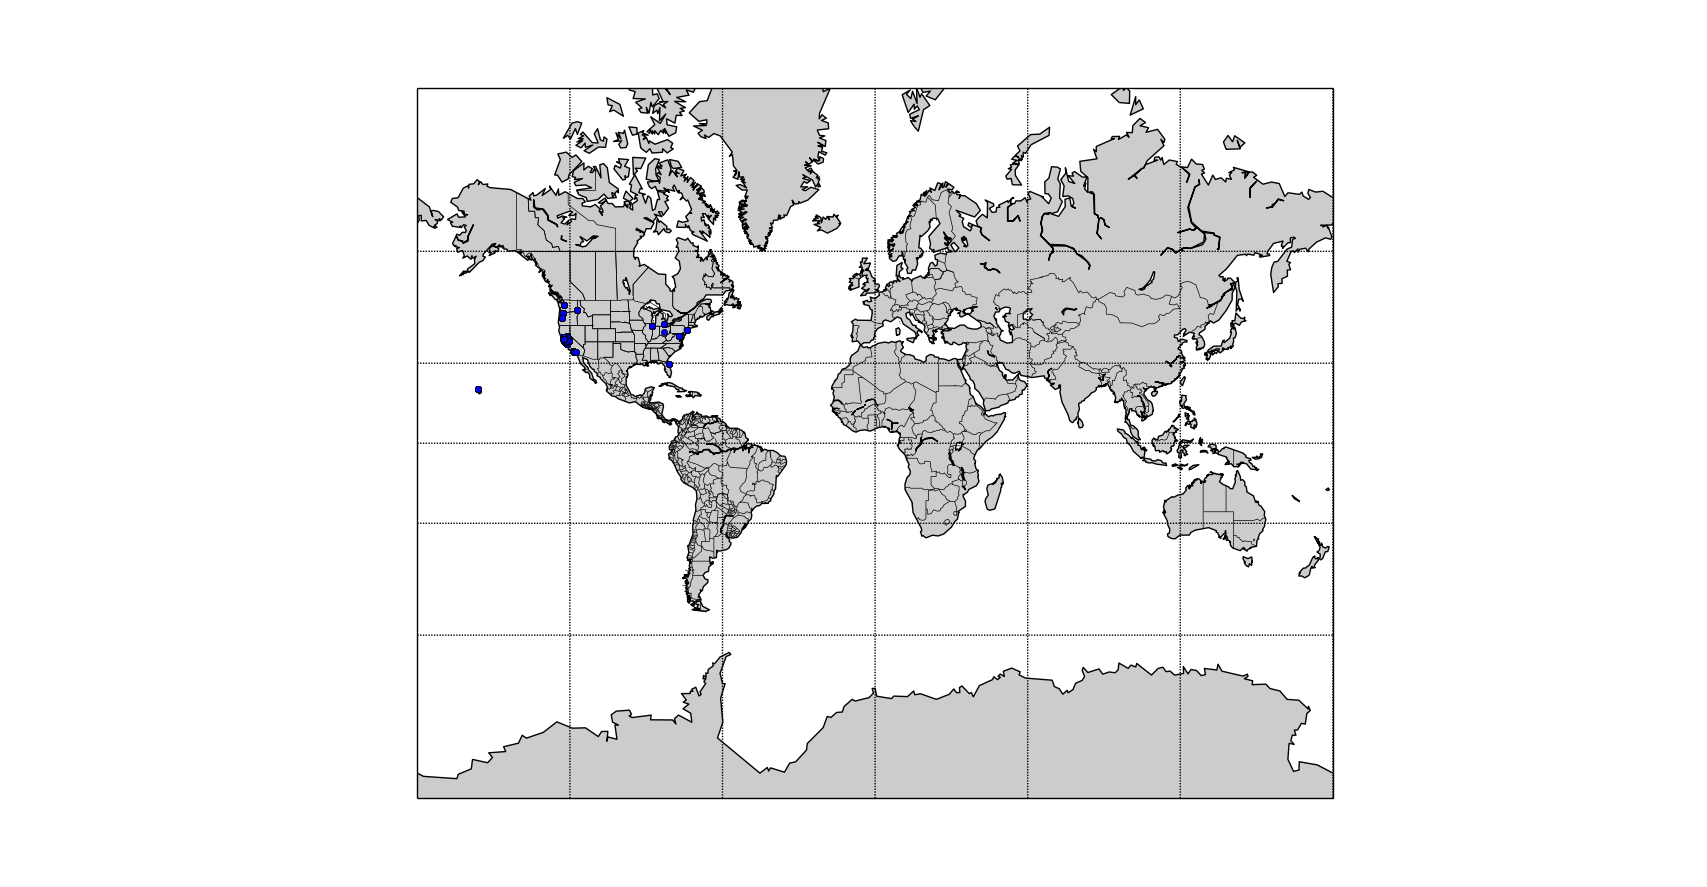
\includegraphics[width=\textwidth]{../home_zips_world.png}
                \caption{On the world map}
                \label{fig:homezips:world}
        \end{subfigure}%
        ~ %add desired spacing between images, e. g. ~, \quad, \qquad, \hfill etc.
          %(or a blank line to force the subfigure onto a new line)
        \begin{subfigure}[b]{0.5\textwidth}
                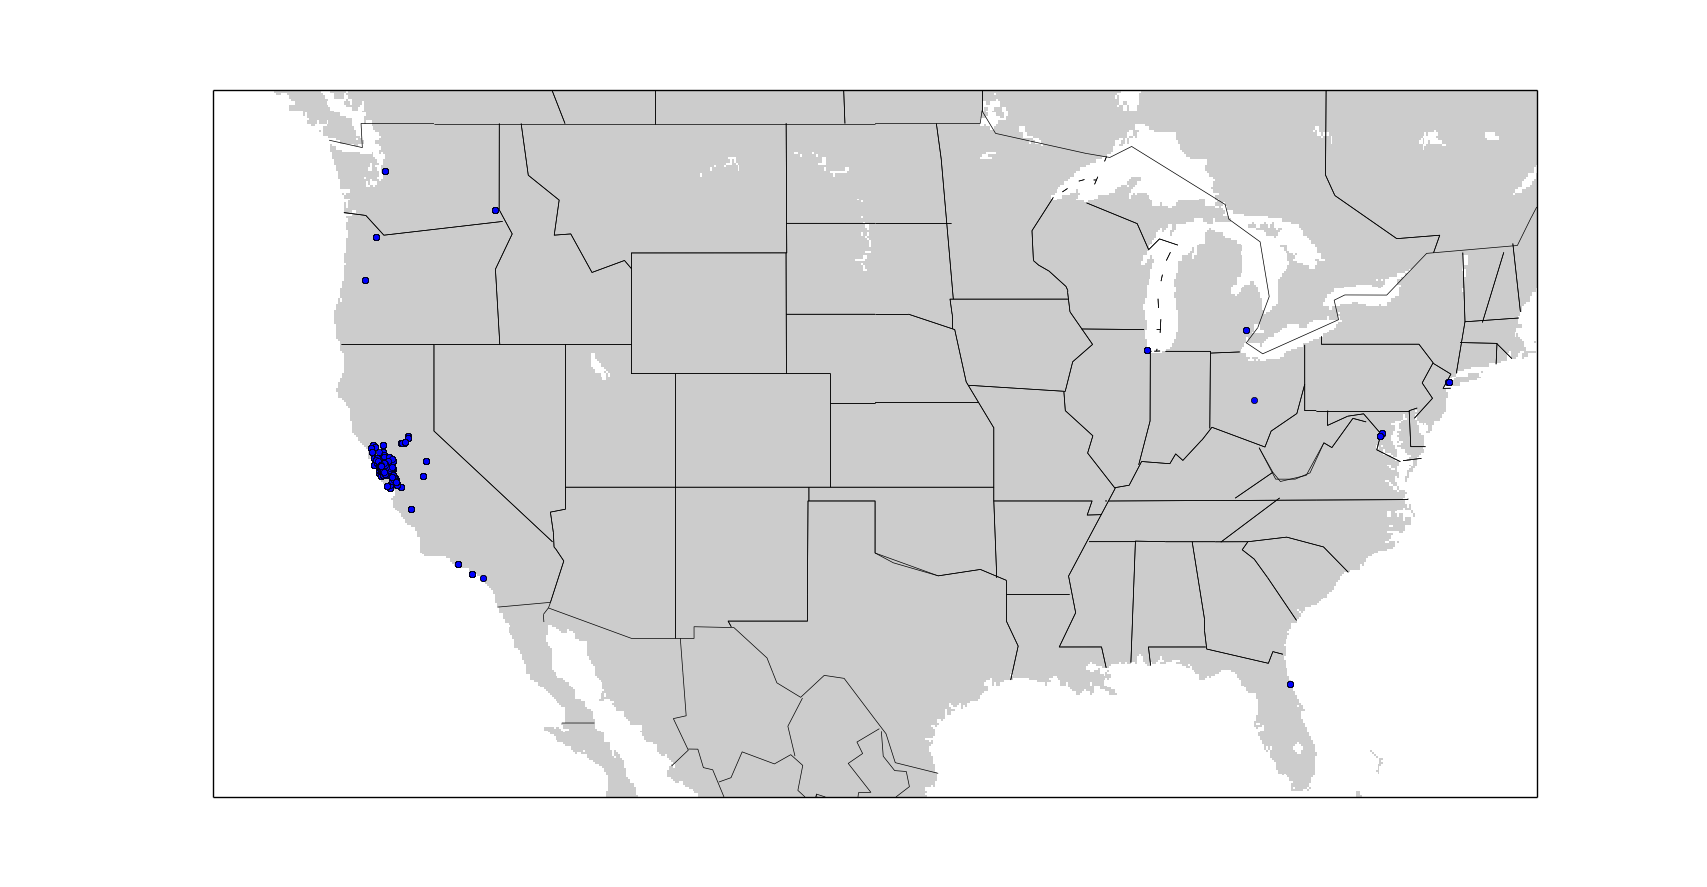
\includegraphics[width=\textwidth]{../home_zips_usa.png}
                \caption{On contiguous states map}
                \label{fig:homezips:usa}
        \end{subfigure}
        ~ %add desired spacing between images, e. g. ~, \quad, \qquad, \hfill etc.
          %(or a blank line to force the subfigure onto a new line)
        \begin{subfigure}[b]{0.4\textwidth}
                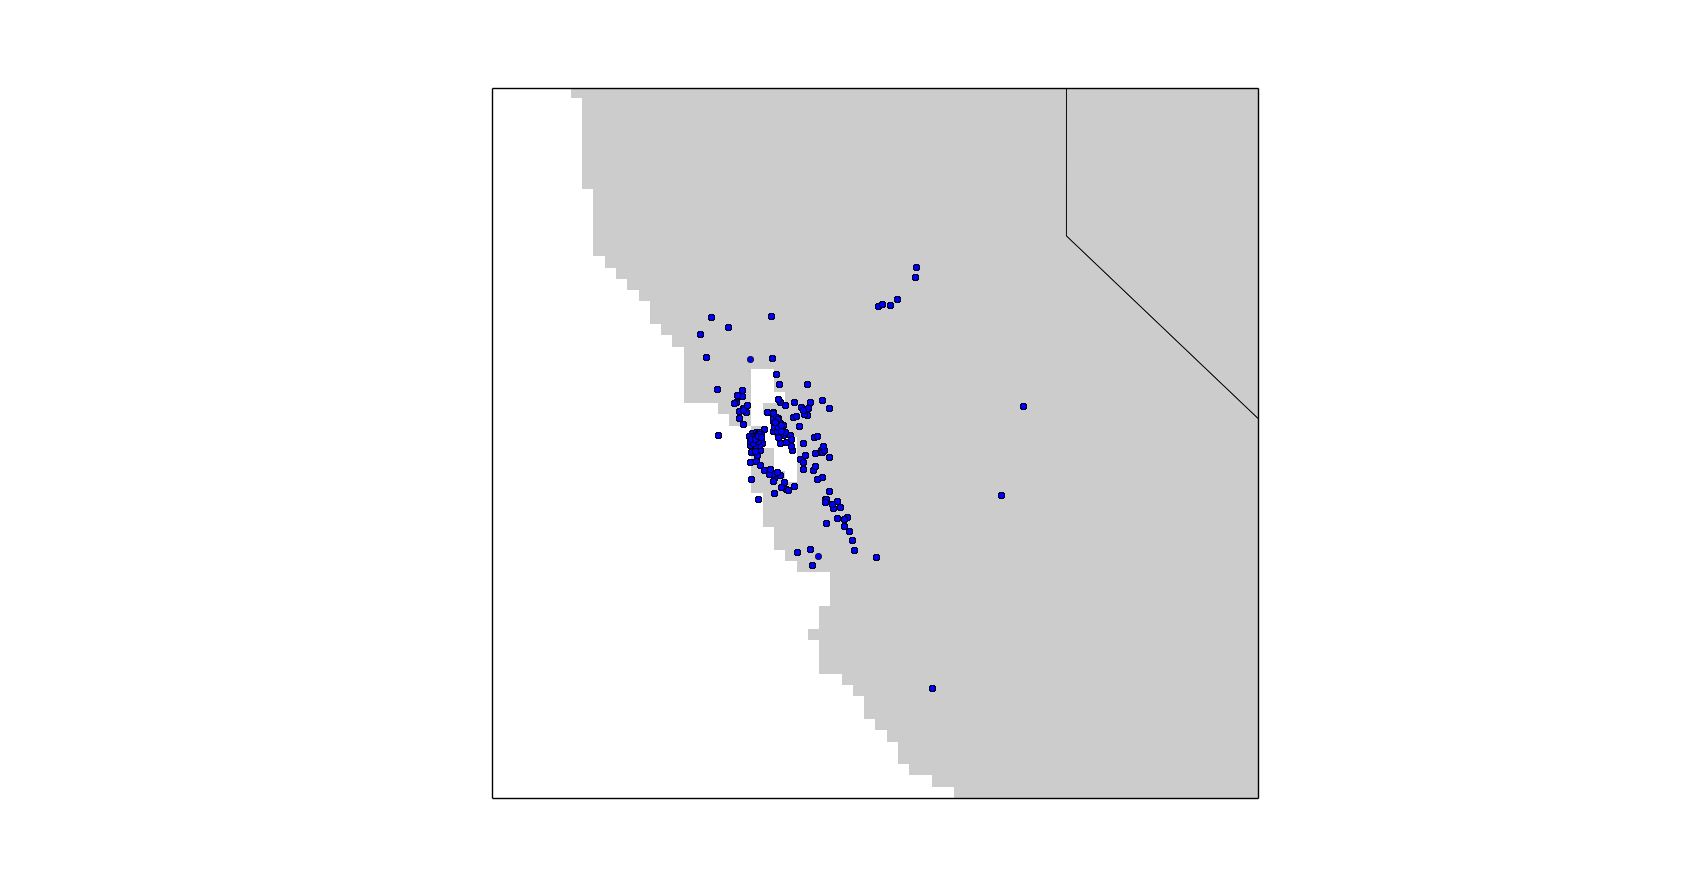
\includegraphics[width=\textwidth]{../home_zips_norcal.png}
                \caption{On Northern California map}
                \label{fig:homezips:norcal}
        \end{subfigure}
        \begin{subfigure}[b]{0.4\textwidth}
                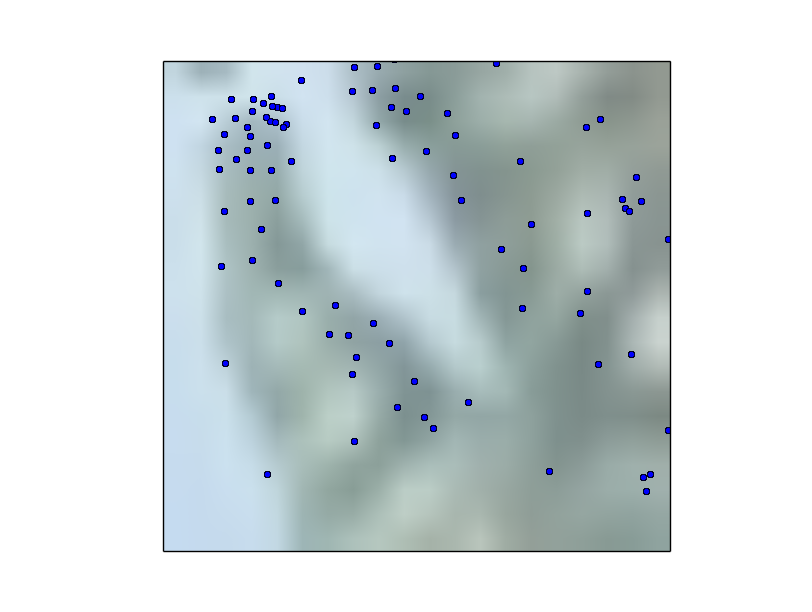
\includegraphics[width=\textwidth]{../home_zips_bay_area.png}
                \caption{On Bay Area map}
                \label{fig:homezips:}
        \end{subfigure}
        \caption{Coordinates of home zip codes of subscribers}
        \label{fig:homezips}
\end{figure}

\begin{figure}
	\centering
	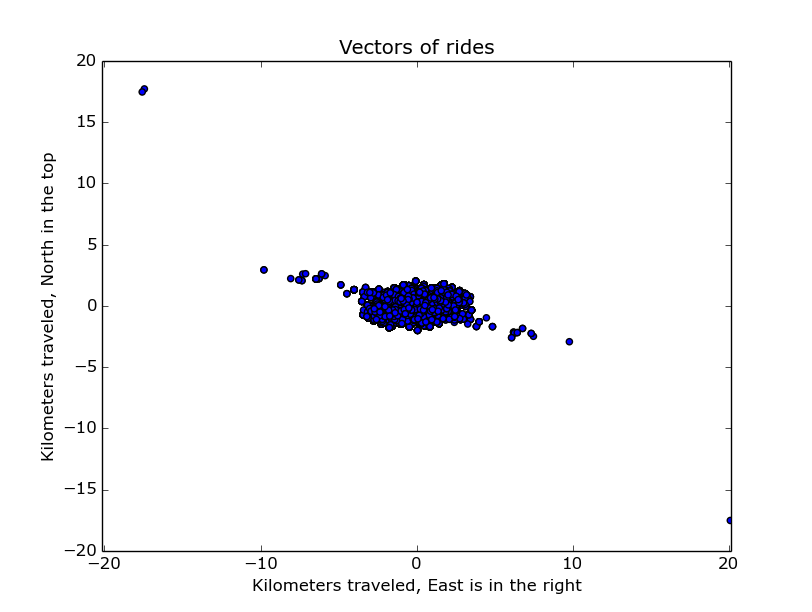
\includegraphics[width=\textwidth]{../travel_vector.png}
	\caption{Distribution of travel vectors, in kilometers}
	\label{fig:travelvector}
\end{figure}

\begin{figure}
	\centering
	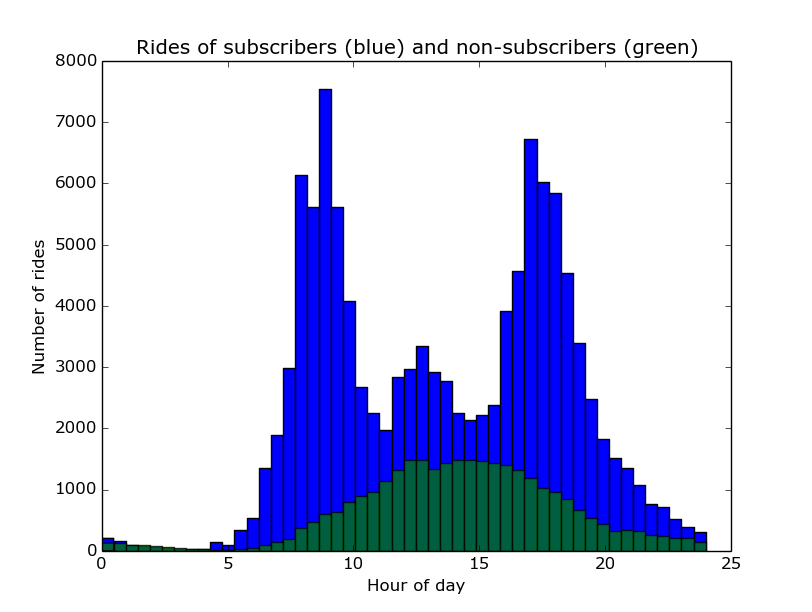
\includegraphics[width=\textwidth]{../time_of_day_sub_not_sub.png}
	\caption{Distribution of travel vectors, in kilometers}
	\label{fig:sns}
\end{figure}



\begin{figure}
	\centering
	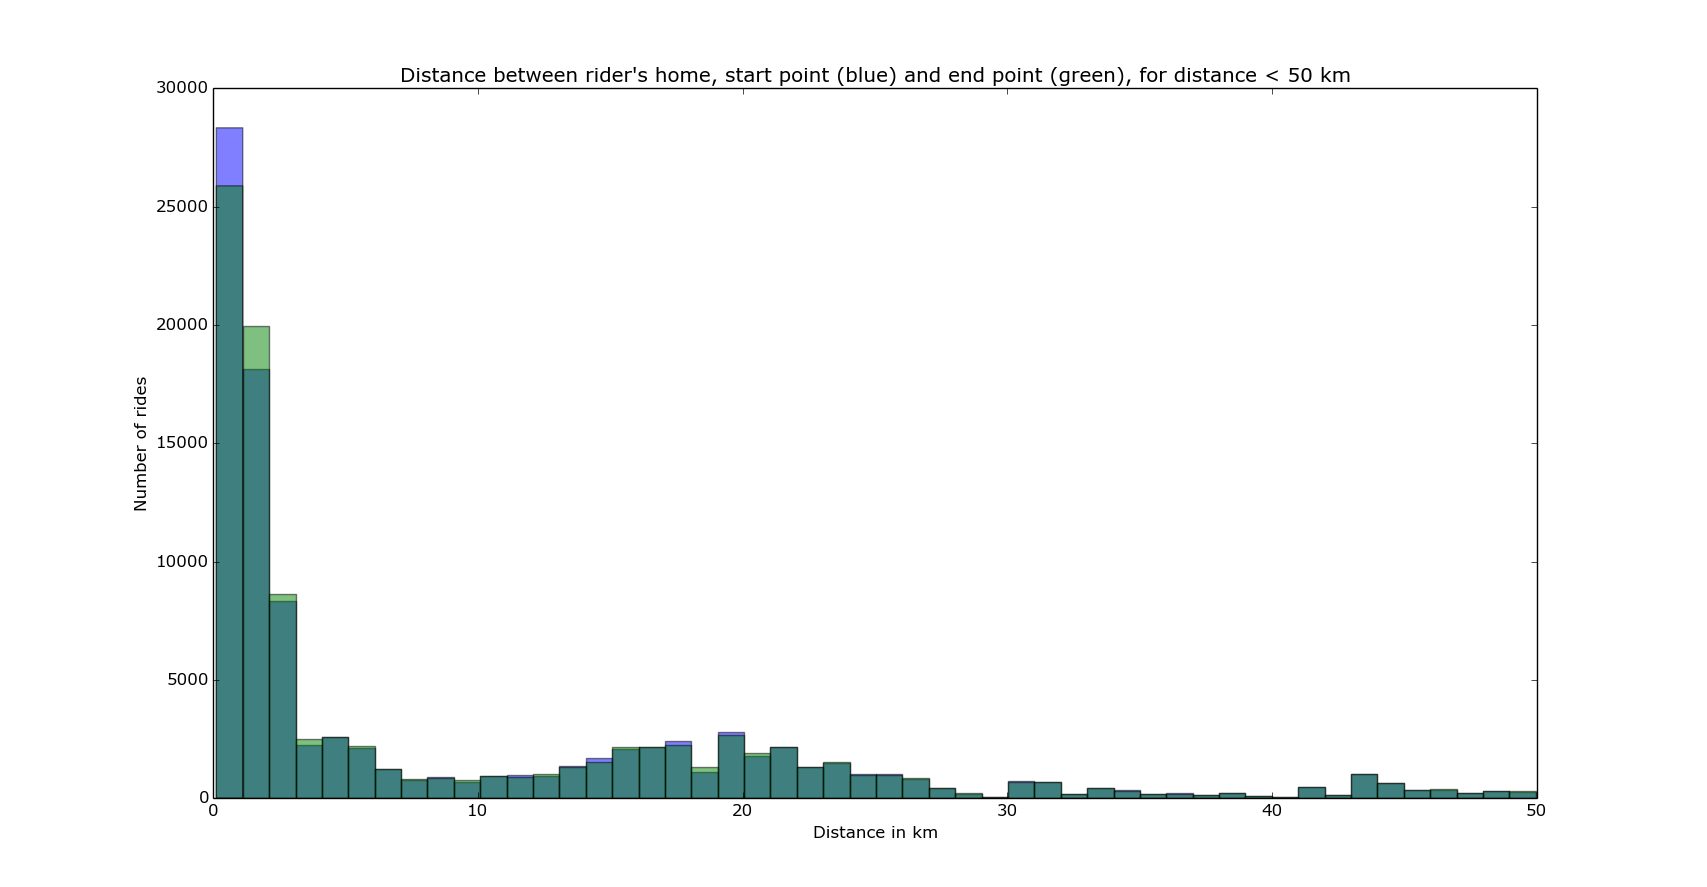
\includegraphics[width=\textwidth]{../start_end_home.png}
	\caption{Distribution of distances from user's home to the start point of the trip (blue) and the end point (green)}
	\label{fig:startendhome}
\end{figure}

\begin{figure}
	\centering
	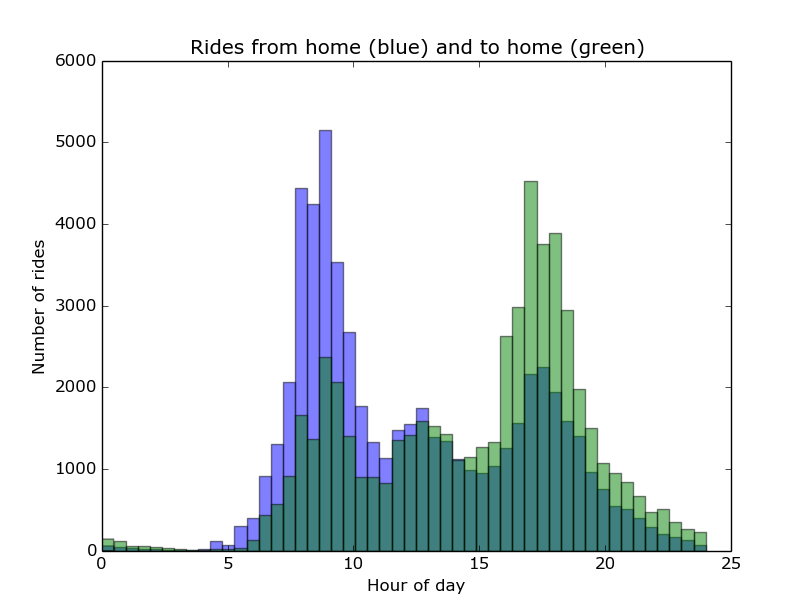
\includegraphics[width=0.8\textwidth]{../rides_from_home_to_home.png}
	\caption{Number of rides per time of the day. Blue are the rides where the user's home is closer to the start point of the ride, and green are the opposite}
	\label{fig:ridestofromhome}
\end{figure}

\begin{figure}
	\centering
	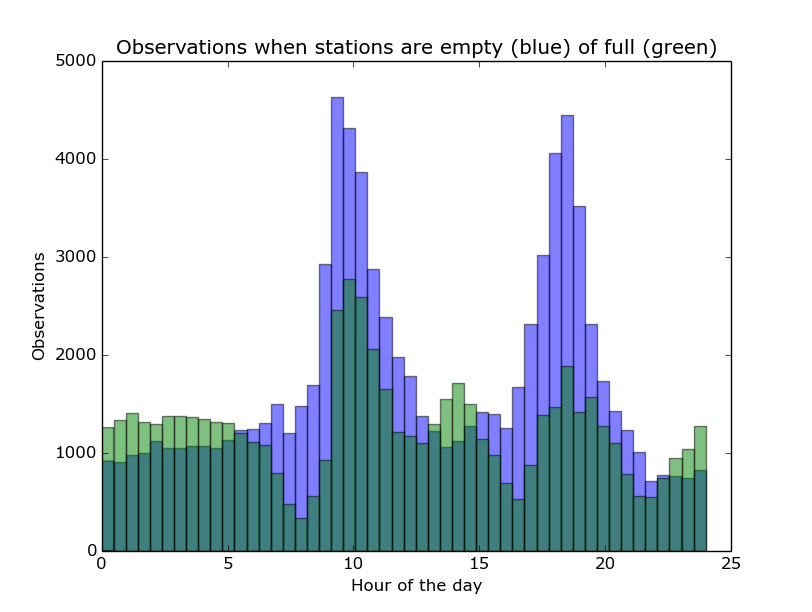
\includegraphics[width=0.8\textwidth]{../empty_full_stations.png}
	\caption{Observations of empty and full stations. Observations are made every minute, so for each bar the height is proportional to the sum of the portions of time each station has stayed empty or full. }
	\label{fig:emptyfull}
\end{figure}


\bibliographystyle{apa}

\begin{thebibliography}{9}

\bibitem{mousebird}
\url{http://mousebirdconsulting.blogspot.ru/2014/04/bay-area-bike-share-data-challenge.html}

\bibitem{planetbabs}
\url{http://www.bayareabikeshare.com/assets/pdf/Bjorn.pdf}

\bibitem{babs}
\url{http://thfield.github.io/babs/}


\end{thebibliography}




\end{document}

